% !TEX root = B99_main.tex


Buildings are a critical element in our modern society and accommodate a variety of needs and functions. Unfortunately the energy consumed by buildings accounts for 32\% of global final energy consumption and 19\% of energy-related greenhouse gas emissions \cite{IPCC}. The existing building stock, therefore, offers a great potential for CO$_2$ mitigation of up to 50\% - 90\% using existing technologies \cite{IPCC}. Of these proposed technologies, building integrated photovoltaics (BIPV) have been recognised as a viable path to supply the energy needs of a building \cite{defaix2012technical,raugei2009life}. \\


%Even the photovoltaic (PV) industry has identified BIPV as one of the four key factors for the future success of PV . 

Developments in efficiency and costs of thin-film BIPV technologies have brought new design possibilities \cite{NREL, kushiya2014cis, kaelin2004low,jelle2012building}. Their lightweight and flexible nature allows for easier and more aesthetically pleasing integration into the building envelope. Furthermore, from a life-cycle perspective, there are attractive returns on embodied energy \cite{perez2012faccade,jayathissa2016life}. One such example is the application of thin film PV on glazed surfaces to create a semi transparent BIPV system \cite{li2009energy,peng2016numerical,vats2012energy}. Such systems not only generate electricity, but also influence the thermo-optic properties of a building, which in Los Angeles can reduce the HVAC energy demand by 30\% \cite{chae2014building}. However, when used in colder climates, the reduction of solar heat gains results in a net HVAC loss \cite{chae2014building}.

Dynamic building envelopes can mitigate this loss by actively controlling direct and indirect radiation into the building, while still responding to the occupant's desires \cite{loonen2013climate}. As seen in Figure \ref{fig:ASFschematic2} this mediation of solar radiation has the potential of improving daylight distribution, while simultaneously reducing heating and cooling demands \cite{nagy2016adaptive}. Using thin film solar panels as our shading element also allows for the simultaneous production of photovoltaic electricity. \\

%In addition, less power is required to actuate them, thus facilitating the development of dynamic envelope elements \cite{nagy2016adaptive, rossi2012adaptive}. \\

%Interestingly, the mechanics that actuate dynamic envelopes couples seamlessly with the mechanics required for facade integrated PV solar tracking. 

Previous research in this field can be divided into two categories: the integration of building energy performance simulation with shading, and the effects of BIPV on building energy performance. 

With respect to the first category, the effects of external shading on building energy performance have been widely studied \cite{bellia2014overview}. Palmero-Marrero et al. analyses the effects of external louvres using TRNSYS \cite{palmero2010effect}. The paper shows that significant energy savings for space cooling is possible in hot climates, however in cities like London, the increase in the heating demand results in a net energetic loss. Nielsen et al. quantified the performance of dynamic solar shading systems using both building thermal and daylight simulations with a case study in Denmark \cite{nielsen2011quantifying}. The results show that a dynamic shading system is the best design alternative as it has an improvement in daylighting performance over fixed shading systems.\ 

Previous BIPV research analyses electricity production and building energy demand for static BIPV shading systems. Freitas et al. analyses different configurations of BIPV systems and shows that a tilted louvre configuration generates 20\% - 40\% more electricity than a flat vertical layout \cite{freitas2015maximizing}. Sun et al. analyses a static tilted photovoltaic system mounted over windows and reports a 51.6\% reduction in cooling demand \cite{sun2012optimum}. Mandalaki et al. expands this analysis to 13 different types of shading devices with integrated PV \cite{mandalaki2012assessment}. Hu et al. combines PV production with building energy performance in an analysis of Trombe wall systems and finds that a Trombe wall with PV venetian blinds has a 45\% energy saving when compared to classic PV Trombe wall systems \cite{hu2017comparative}. Optimising the panel angles for PV production however are not always advantageous. Chatzipanagi et al. demonstrated that an inclination of 30$^{\circ}$ of integrated crystaline modules results in very high operating temperatures, thus penalising the system \cite{chatzipanagi2016bipv}. It is therefore important to also include thermal effects in BIPV analysis. \\

%\added[id=pj, remark=``This version was created based on Zoltans comments on the previous iteration'']{V1: We have previously combined the two aforementioned categories to evaluate the annual performance of a dynamic photovoltaic shading system and its impact on the building energy demand \cite{jayathissa2016PVSEC}. The methodology was sufficient to attain an understanding of how such a system functions, however it used simplifications that ignored time dependant characteristics of the building, such as thermal capacitance. This paper expands on this previous research in two parts. Firstly, by running hourly simulations that combine the electricity production of the dynamic shading system with the building energy demand. Secondly, by proposing a novel adaptive control strategy where the results of each hourly simulation are used to determine the orientation of the PV panels. By doing so, we can not only evaluate the hourly performance of an adaptive photovoltaic shading system, but can also use the same framework to control the physical system.}\\

This paper expands on this previous research in two parts. Firstly, by combining the two aforementioned categories to evaluate a dynamic photovoltaic shading system and its interaction with the building energy demand. Secondly, by proposing a novel adaptive control strategy where the results of the simulation are used to determine the orientation of the PV panels. We have previously modelled the energy performance of dynamic BIPV shading systems \cite{jayathissa2016PVSEC}. The methodology was sufficient to attain an understanding of how such a system functions, however it used simplifications that ignored time-dependent characteristics of the building, such as thermal capacitance. \\


The contribution of this paper is a simulation framework that overcomes these simplifications, in order to evaluate the energetic performance of adaptive photovoltaic envelopes with respect to PV electricity production and building energy demand. We apply the framework in this paper in the context of the Adaptive Solar Facade (ASF) project, shown in Figure \ref{fig:HoNR2} \cite{nagy2016adaptive}. The ASF is a lightweight PV shading system composed of dynamically actuated copper indium gallium selenide (CIGS) panels. CIGS panels from Flisom were chosen due to their light-weight nature, high efficiency, and monolithic interconnection, however in principle any light-weight PV material can be used \cite{feurer2016progress}. Each panel can independently rotate in two degrees of freedom, through the use of a soft pneumatic actuator \cite{svetozarevic2016soro}. This freedom enables local variations of the facade when reacting to internal and external factors.  For more information on the technology, please refer to the publication by Nagy et al. \cite{nagy2016adaptive}.\\

%CIGS panels were chosen due to their light-weight nature, efficiency, and availability of a local supplier, however in principle any light-weight PV material can be used. 
%This paper expands on this work by analysing dynamic PV shading systems, while also taking into account mutual shading amongst modules and its effect on PV electricity generation. This approach allows us to reduce efficiency degradation due to partial shading of PV modules \cite{hofer2016parametric}.
%


%Attempts to model a dynamic PV shading system was first presented at the EUPVSEC 2016 \cite{jayathissa2016PVSEC}, which provides a general understanding of dynamic BIPV systems, but uses simplifications which ignore transient characteristics of the building, such as thermal capacitance. \\

% Attempts to analyse dynamic BIPV systems have still been conducted through static simulations where every possible configuration of an adaptive envelope is computed for every hour of the year, followed by a post processing algorithm which extracts the best configuration for each hour \cite{jayathissa2016PVSEC}. Although this method is good to gain a general understanding of dynamic BIPV systems, it lacks transient characteristics of the buildings behaviour, such as thermal capacitance. \\

%A high-resolution radiation analysis is conducted through a parametric Rhino/Grasshopper environment \cite{grasshopper}. The results are then coupled to a resistance - capacitance (RC) model  to determine the energy consumption of the building \cite{de2008iso}. This methodology ultimately enables us to assess the performance of dynamic BIPV and investigate control strategies for future application. \\

% We also include more complex physics within our radiation analysis such as the effects of mutual shading amongst modules \cite{hofer2016parametric}. 




The remainder of the paper is organised as follows. The next section describes the simulation methodology including the case study used in the analysis. In Section \ref{ch:results2} we present the results of the case study which describes the adaptive response of the ASF to variations in the external and internal environment. Finally, Section \ref{ch:conclusion2} concludes the paper.


% This paper expands on this work by analysing dynamic PV shading systems, while also taking into account mutual shading amongst modules and its effect on PV electricity generation. The approach allows us to reduce efficiency degradation due to partial shading of PV modules \cite{hofer2015PVSEC}.

 


% Within this study we analyse the trade-off in winter between PV generation and heating the room through solar insolation. Likewise in summer we discuss the trade-off between cooling and natural lighting. 

% The state of the art in this field is restricted to static shading devices \cite{yoo2011available} \cite{mandalaki2012assessment}. This paper presents a methodology to simulate a dynamic solar facade and calculate the electricity production in combination with the energy consumption of the building. 


\begin{figure}
\begin{center}
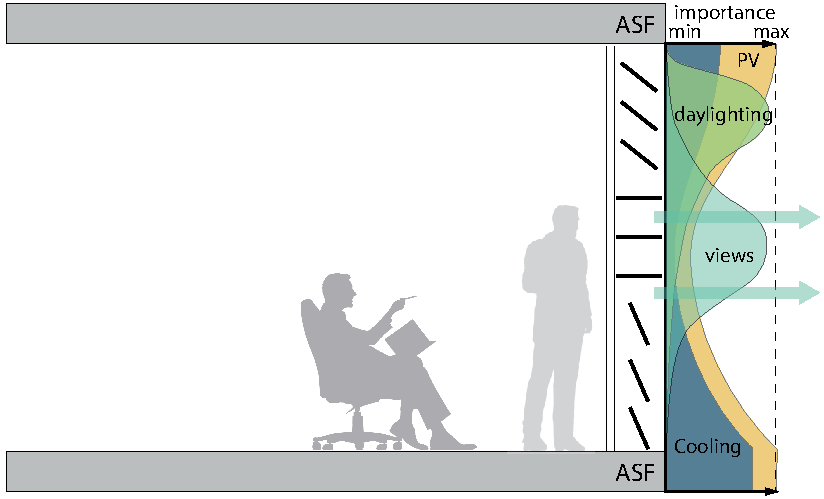
\includegraphics[width=8cm, trim= 0cm 0cm 0cm 0cm,clip]{facadeFunctionsnew.pdf}
\caption{The facade acting as a mediator between the interior and exterior environment, while fulfilling various functions \cite{nagy2016adaptive}}
\label{fig:ASFschematic2}
\end{center}
\end{figure}

\begin{figure}
\begin{center}
\includegraphics[width=8cm, trim= 0cm 0cm 0cm 0cm,clip]{honr.jpg}
\caption{An example of an ASF constructed at the House of Natural Resources \cite{nagy2016adaptive}}
\label{fig:HoNR2}
\end{center}
\end{figure}




